\newvideofile{kondensator}{Kondensatornetzwerke}
\newpage



\begin{frame}

	\section{Einfache Kondensatornetzwerke}
	\s{
	
		Wie Widerstände lassen sich auch Kapazitäten zu Netzwerken zusammenschließen. Die einfachen Grundschaltungen, welche 
		wiederum zu beliebig komplexen Netzwerken zusammengeschaltet werden können, werden nachfolgend vorgestellt. 
		
		\subsection{Parallelschaltung von Kapazitäten}
		
		Sind in einer Schaltung mehrere Kapazitäten parallel zueinander geschaltet, lassen sie sich zu einer
		Gesamtkapazität zusammenfasssen (siehe Abbildung \ref{fig:parallelkondensator}).
		
		
		\begin{figure}[h!]
			\begin{center}

				\begin{tikzpicture}
    \draw(0,0) to[short] (2,0)
    to[C, i, v<, name=C1, l =$C_1$] (2,2)
    to[short](4.5,2)
    %to[C, i, v>, name=C2] (5,0)
    to[short](0,2)
    to[short](0,0)
    to[V, v<, i, name=V1] (0,2)
    to[short](2,2);
    \draw(4.5,0)to[C, i, v<, name=C2, l =$C_2$] (4.5,2);
    \draw(4.5,0)to[short] (2,0);


    \varrmore{V1}{$U_0$};
    \varrmore{C1}{$U_1$};
    \varrmore{C2}{$U_2$};

    \draw[thick] (6.2,1.0) -- (6.075,1.125) -- (6.075,1.05) -- (5.825,1.05) -- (5.825,1.125) -- (5.7,1.0) -- (5.825,0.875) -- (5.825,0.95) -- (6.075,0.95) -- (6.075,0.875) -- cycle;

    \draw(7.5,0) to[short] (9.5,0)
    to[C, i, v<, name=C12, l =$C_\mathrm{ges}$] (9.5,2)
    to[short](9.5,2)
    %to[C, i, v>, name=C2] (12.5,0)
    to[short](7.5,2)
    to[short](7.5,0)
    to[V, v<, i, name=V12] (7.5,2)
    to[short](9.5,2);


    \varrmore{V12}{$U_0$};
    \varrmore{C12}{$U_0$};
\end{tikzpicture}
				
			\end{center}
			\label{fig:parallelkondensator}
			\caption{Zusammenfassen von zwei parallel geschalteten Kapazitäten $C_1$ und $C_2$ zu einer Gesamtkapazität $C_\mathrm{ges}$}
		\end{figure}
		
		Dabei liegt an allen Einzelkapazitäten die gleiche Spannung an:
		
		\begin{equation*}
			U_0 = U_1 = U_2
		\end{equation*}
		
		Die Ladung, welche auf jedem der Einzelkondensatoren gespeichert ist, kann wie folgt bestimmt werden:
		
		\begin{equation*}
			Q_k = C_k \cdot U_0
		\end{equation*}
		
		Die Gesamtladung $C_\mathrm{ges}$ auf dem in Abbildung \ref{fig:parallelkondensator} Ersatzschaltbild entsprechend mit
		
		\begin{equation*}
			Q_\mathrm{ges} = C_\mathrm{ges} \cdot U_0
		\end{equation*}
		
		Die Gesamtladung setzt sich aus der Summe der Einzelladungen zusammen:
		
		
		\begin{equation*}
			Q_\mathrm{ges} = Q_1 + Q_2 = C_1 \cdot U_0 + C_2 \cdot U_0 
		\end{equation*}
		
		
		
		\begin{equation*}
			Q_\mathrm{ges} =  (C_1 + C_2) \cdot U_0 
		\end{equation*}
		
		Ein Quotientenvergleich mit der ursprünglichen Berechnung der Gesamtladung $Q_\mathrm{ges}$ zeigt nun:
		
		
		
		\begin{equation*}
			\rightarrow C_1 + C_2 = C_\mathrm{ges}
		\end{equation*}
		
		Auch für beliebig viele parallelgeschaltete Kapazitäten gilt, dass die Summe der Einzelkapazitäten die Gesamtkapazität ergibt:
		
		
		\begin{Merksatz}{Gesamtkapazität einer Parallelschaltung}
			
			\begin{equation*}
				C_\mathrm{ges} = \sum_{k=1}^{n} C_k 
			\end{equation*}
			
		\end{Merksatz}
		
	}
	
	
	
	\b{
		\ftx{Parallelschaltung von Kapazitäten}
		\begin{columns}
			\column[t]{0.5\textwidth}
			\vspace*{-110pt}
			
			\textbf{Parallelschaltung}: Spannung aller Kapazitäten identisch: \\
			
			\vspace*{-10pt}
			\begin{equation*}
				U_0 = U_1 = U_2	
			\end{equation*}
			
			Ladung pro Kondensator:
			\begin{equation*}
				Q_k = C_k \cdot U_k, \quad Q_\mathrm{ges} = C_\mathrm{ges} \cdot U_0
			\end{equation*}
			
			\visible<2->{
				Gesamtladung $Q_\mathrm{ges}$:
				
				\vspace*{-5pt}
				
				\begin{equation*}
					Q_\mathrm{ges} = Q_1 + Q_2 = C_1 \cdot U_0 + C_2 \cdot U_0 
				\end{equation*}
				\vspace*{-15pt}
				\begin{equation*}
					Q_\mathrm{ges} =  (C_1 + C_2) \cdot U_0 
				\end{equation*}
				\vspace*{-20pt}
				
				\begin{equation*}
					\rightarrow C_1 + C_2 = C_\mathrm{ges}
				\end{equation*}
			}
			
			
			\column[c]{0.5\textwidth}
			
			
			
			\begin{tikzpicture}
				\draw(0,0) to[short] (2,0)
				to[C, i, v<, name=C1, l =$C_1$] (2,2)
				to[short](4.5,2)
				%to[C, i, v>, name=C2] (5,0)
				to[short](0,2)
				to[short](0,0)
				to[V, v<, i, name=V1] (0,2)
				to[short](2,2);
				\draw(4.5,0)to[C, i, v<, name=C2, l =$C_2$] (4.5,2);
				\draw(4.5,0)to[short] (2,0);
				
				
				\varrmore{V1}{$U_0$};
				\varrmore{C1}{$U_1$};
				\varrmore{C2}{$U_2$};
				
			\end{tikzpicture}
			
			% \vspace*{5pt}
			\begin{center}


				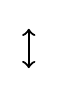
\begin{tikzpicture}
					\draw[<->, thick] (0,0) -- (0,0.5);
				\end{tikzpicture}
				
				\vspace*{5pt}
				
				
				\begin{tikzpicture}
					\draw(0,0) to[short] (2,0)
					to[C, i, v<, name=C1, l =$C_\mathrm{ges}$] (2,2)
					to[short](2,2)
					%to[C, i, v>, name=C2] (5,0)
					to[short](0,2)
					to[short](0,0)
					to[V, v<, i, name=V1] (0,2)
					to[short](2,2);
					
					
					\varrmore{V1}{$U_0$};
					\varrmore{C1}{$U_0$};
					
					
				\end{tikzpicture}
				
			\end{center}
			\vspace*{-15pt}
			
			
			\visible<2->{
				\begin{Merksatz}{}
					
					\begin{equation*}
						C_\mathrm{ges} = \sum_{k=1}^{n} C_k 
					\end{equation*}
					
				\end{Merksatz}
			}
		\end{columns}
		
		\speech{folie27}{1}{Die an Widerstandsnetzwerken durchgeführten Betrachtungen können wir analog auch für Kapazitäten durchführen. Wie Widerstände lassen sich auch Kapazitäten zu
			Netzwerken zusammenschließen.
			Beginnen wir mit der Parallelschaltung von zwei Kapazitäten, welche wir zu einer Gesamtkapazität zusammenfassen wollen. 
			Dabei liegt auch hier an allen Einzelkapazitäten die gleiche Spannung an. Das bedeutet:
			U 0 gleich U 1 gleich U 2.
			Die Ladung, welche auf jedem der Einzelkondensatoren gespeichert ist, kann für jeden einzelnen Kondensator also über Q gleich C mal U bestimmt werden.}
			\silence{2}
		\speech{folie27}{2}{Entsprechend kann die Gesamtladung mit Hilfe des Ausdrucks Q gesamt ist gleich C gesamt mal U0 bestimmt werden.
			Die Gesamtladung setzt sich aus der Summe der Einzelladungen zusammen. Für das Beispiel bedeutet das Q gesamt ist gleich Q eins plus Q zwei.
			Daraus folgt Q gesamt ist gleich C1 mal U null plus C2 mal U null.
			Auch hier können wir die Kapazität ausklammern, wodurch sich Q gesamt gleich C1 plus C2 mal U null ergibt.
			Ein Quotientenvergleich mit der ursprünglichen Berechnung der Gesamtladung Q gesamt zeigt nun, das C1 plus C2 gleich C gesamt ist. 
			Also gilt auch für beliebig viele parallelgeschaltete Kapazitäten, dass die Summe der Einzelkapazitäten die Gesamtkapazität ergibt.}
			\silence{4}
		
	}
	
\end{frame}


%	\begin{frame}
%		\fta{Reihenschaltung von Induktivitäten}
%		\begin{columns}
%			\column[t]{0.5\textwidth}
%			\vspace{-60pt}
%			\phantom{.}\\
%
%			Bei der Zusammenschaltung mehrerer Spulen in Reihe
%			werden alle Induktivitäten von dem gleichen Strom durchflossen. \\
%			\phantom{.} \\
%			Aus dem Spannungsumlauf erhält man die Gleichung: \\
%			$u_\mathrm{ges} = \sum_{k=1}^{n} u_k = \sum_{k=1}^{n} L_k \frac{di}{dt} = L_\mathrm{ges} \cdot \frac{di}{dt}$ \\
%		   

%			Die gesamte an den Eingangsklemmen wirksame Induktivität ist durch die Summe der einzelnen Induktivitäten gegeben. \\




%			   \begin{tikzpicture}
%				\draw(0,0) to[short] (4,0)
%					 to[L=$L_2$,v<,name=L2] (4,2)
%					 to[L=$L_1$,v<,name=L1] (4,4)
%					 to[short](0,4)
%					 to[V,v,i,name=U_ges] (0,0);
%
%					 \varrmore{L1}{$U_1$};
%					 \varrmore{L2}{$U_2$};
%					 \varrmore{U_ges}{$U_\mathrm{ges}$};
%					 \iarrmore{U_ges}{$I_\mathrm{ges}$};
%			   \end{tikzpicture} \\
%
%			   \phantom{.} \\
%			   \phantom{.} \\
%	 
%			   \phantom{.} \\
%	 
%			   \begin{Merksatz}{}
%				$L_\mathrm{ges} = \sum_{k=1}^{n} L_k$
%			   \end{Merksatz}
%			   
%			  
%	 
%			\end{columns}
%		   
%	 
%	   
%		\end{frame}


\begin{frame}

	\subsection{Reihenschaltung von Kapazitäten}
	
	\s{
		Bei der Reihenschaltung von Kapazitäten teilt sich die gesamte an den Eingangsanschlüssen anliegende 
		Spannung $U_\mathrm{0}$ in die Teilspannungen $U_k$ an den einzelnen Kapazitäten auf (Abbildung \ref{fig:kondensatorreihe}). \\
		
		
		
		
		
		\begin{figure}[h!]
			\begin{center}

				\begin{tikzpicture}
    \draw(0,0) to[short, o-] (0.5,0)
    to[C, i, v<, name=C2, l =$C_2$] (2.5,0)
    to[short](3,0)
    to[short](3,3)
    to[short](2.5,3)
    to[C, i, v<, name=C1, l =$C_1$] (0.5,3)
    to[short, -o](0,3);

    \varrmore{C1}{$U_1$};
    \varrmore{C2}{$U_2$};
    \draw[->, thick, voltage] (0,2.8) -- (0,0.2) node[midway,left] {$U_0$};

    \draw[thick] (3.85,1.5) -- (3.725,1.625) -- (3.725,1.55) -- (3.475,1.55) -- (3.475,1.625) -- (3.35,1.5) -- (3.475,1.375) -- (3.475,1.45) -- (3.725,1.45) -- (3.725,1.375) -- cycle;

    \draw(4.8,0) to[short, o-] (6,0)
    to[short](6,0.5)
    to[C, i, v<, name=Cges, l_ =$C_\mathrm{ges}$] (6,2.5)
    to[short](6,3)
    to[short, -o](4.8,3);

    \draw[->, thick, voltage] (4.7,2.8) -- (4.7,0.2) node[midway,left] {$U_0$};

    \node at (0.9,2.7) {$+Q$};
    \node at (2,2.7) {$-Q$};

    \node at (0.9,0.3) {$+Q$};
    \node at (2,0.3) {$-Q$};

    \node at (5.55,1.9) {$+Q$};
    \node at (5.55,1.1) {$-Q$};


\end{tikzpicture} \\
			\end{center}
			\label{fig:kondensatorreihe}
			
			\caption{Zusammenfassen von zwei in Reihe geschalteten Kapazitäten $C_1$ und $C_2$ zu einer Gesamtkapazität $C_\mathrm{ges}$}
			
			
			
			
		\end{figure}
		
		
		
		Auf den jeweils mit den Anschlussklemmen verbundenen Kondensatorplatten wird eine Ladung $\pm \, Q$ aufgeprägt.
		Beide Platten des selben Kondensators haben stets betragsgleiche Ladungen, was dazu führt, dass beide Kondensatoren an den Anschlussklemmen
		der Reihenschaltung auf beiden Platten die Ladung $\pm \, Q$ haben. Die äußere Platte des jeweils nächsten angeschlossenen Kondensators
		muss betragsmäßig identisch mit umgekehrten Vorzeichen geladen sein, da aus der ursprünglich elektrisch neutralen Verbindung keine 
		Ladungsträger entweichen oder hinzugefügt werden können. Diesem Schema folgend besitzen alle Kondensatoren
		einer Reihenschaltung die gleiche Ladung $Q$.
		
		Ausgehend von der Kondensator-Grundgleichung $Q = C \cdot U$ ergibt sich für die Teilspannungen, welche an den
		in Abbildung \ref{fig:kondensatorreihe} gezeigten Kondensatoren abfallen:
		
		\begin{equation*}
			U_1 = \frac{Q}{C_1}, \quad \quad U_2 = \frac{Q}{C_2}
		\end{equation*}
		
		Eingesetzt in das Ergebnis des Maschenumlaufs der Ausgangsschaltung ergibt sich:
		
		\begin{equation*}
			U_0 = U_1 + U_2 = \left( \frac{1}{C_1} + \frac{1}{C_2} \right) \cdot Q
		\end{equation*}
		
		Die Spannung $U_0$ im Ersatzschaltbild kann wie folgt berechnet werden:
		
		\begin{equation*}
			U_0 = \frac{1}{C_\mathrm{ges}} \cdot Q
		\end{equation*}
		
		Ein Quotientenvergleich offenbart:
		
		\begin{equation*}
			\frac{1}{C_1} + \frac{1}{C_2} = \frac{1}{C_\mathrm{ges}}
		\end{equation*}
		
		Allgemein gilt für eine Reihenschaltung aus beliebig vielen Kondensatoren:
		
		\begin{Merksatz}{Gesamtkapazität einer Reihenschaltung:}
			\begin{equation}
				\frac{1}{C_\mathrm{ges}} = \sum_{i = 1}^{n} \frac{1}{C_i}
			\end{equation}
		\end{Merksatz}
		
		
		Bei zwei in Reihe geschalteten Kondensatoren kann die Gesamtkapazität $C_\mathrm{ges}$ analog zur 
		Parallelschaltung von Widerständen auch mit folgendem Ausdruck ermittelt werden:\\
		
		\begin{equation*}
			C_\mathrm{ges} = \frac{C_1 \cdot C_2}{C_1 + C_2}
		\end{equation*}

		
	}
	
	
	
	\b{
		\ftx{Reihenschaltung von Kapazitäten}
		\begin{columns}
			\column[t]{0.45\textwidth}
			%\vspace*{-80pt}
			
			\vspace{-110pt}
			
			\textbf{Reihenschaltung}: alle Kondensatoren besitzen \textbf{gleiche Ladung} $Q$!\\
			
			\vspace*{5pt}
			
			Kondensator-Grundgleichung:
			
			\begin{equation*}
				Q= C \cdot U
			\end{equation*}
			\vspace*{-10pt}
			\begin{equation*}
				U_1 = \frac{Q}{C_1}, \quad U_2 = \frac{Q}{C_2}
			\end{equation*}
			
			Reihenschaltung aus Kapazitäten:
			\vspace*{-10pt}
			
			\begin{equation*}
				U_0 = U_1 + U_2 = \bigg( \frac{1}{C_1} + \frac{1}{C_2} \bigg) \cdot Q
			\end{equation*}
			
			Ersatzschaltbild:
			
			\vspace*{-10pt}
			
			\begin{equation*}
				U_0 = \frac{1}{C_\mathrm{ges}} \cdot Q
			\end{equation*}
			
			\column[c]{0.55\textwidth}
			\begin{tikzpicture}
				\draw(0,0) to[short, o-] (0.5,0)
				to[C, i, v<, name=C2, l =$C_2$] (2.5,0)
				to[short](3,0)
				to[short](3,3)
				to[short](2.5,3)
				to[C, i, v<, name=C1, l =$C_1$] (0.5,3)
				to[short, -o](0,3);
				
				\varrmore{C1}{$U_1$};
				\varrmore{C2}{$U_2$};
				\draw[->, thick, voltage] (0,2.8) -- (0,0.2) node[midway,left] {$U_0$};
				
				\draw[thick] (3.85,1.5) -- (3.725,1.625) -- (3.725,1.55) -- (3.475,1.55) -- (3.475,1.625) -- (3.35,1.5) -- (3.475,1.375) -- (3.475,1.45) -- (3.725,1.45) -- (3.725,1.375) -- cycle;
				
				\draw(4.8,0) to[short, o-] (6,0)
				to[short](6,0.5)
				to[C, i, v<, name=Cges, l_ =$C_\mathrm{ges}$] (6,2.5)
				to[short](6,3)
				to[short, -o](4.8,3);
				
				\draw[->, thick, voltage] (4.7,2.8) -- (4.7,0.2) node[midway,left] {$U_0$};
				
				\node at (0.9,2.7) {$+Q$};
				\node at (2,2.7) {$-Q$};
				
				\node at (0.9,0.3) {$-Q$};
				\node at (2,0.3) {$+Q$};
				
				\node at (5.55,1.9) {$+Q$};
				\node at (5.55,1.1) {$-Q$};
				
				
			\end{tikzpicture} \\
			
			\vspace*{-10pt}
			\begin{Merksatz}{}
				
				\begin{equation*}
					\frac{1}{C_\mathrm{ges}} = \sum_{k=1}^{n} \frac{1}{C_k}
				\end{equation*}
				
			\end{Merksatz}
			
		\end{columns}
		
		\speech{folie29}{1}{Bei der Reihenschaltung von Kapazitäten teilt sich die gesamte an den Eingangsanschlüssen anliegende Spannung U null in die Teilspannungen U K an den einzelnen Kapazitäten auf.
			Auf den jeweils mit den Anschlussklemmen verbundenen Kondensatorplatten wird eine Ladung Q aufgeprägt. Hierbei besitzen alle Kondensatoren, die in Reihe geschaltet sind, 
			die betragsmäßig gleiche Ladung Q auf ihren Kondensatorplatten.  
			Ausgehend von der Kondensatorgrundgleichung Q gleich C mal U ergibt sich für die Teilspannungen: 
			U1 gleich Q durch C1 und U2 gleich Q durch C zwei..}
			\silence{2}
			\speech{folie29}{1}{Mit Hilfe der Maschenregel gilt: U0 gleich U 1 plus U 2. Setzen wir hier die Teilspannungen ein und klammern die Ladung Q aus, so ergibt sich:
			U0 gleich 1 durch C1 plus 1 durch C2 mal Q.
			Zusammengefasst gilt also U0 gleich 1 durch C gesamt mal Q.
			Allgemein lässt sich die Gesamtkapazität einer Reihenschaltung über die Summe der Kehrwerte der Einzelkapazitäten bestimmen: 
			1 durch C gesamt ist gleich die Summe der Kehrwerte der Einzelkapazitäten.
			Zusammenfassend lässt sich also sagen, dass man eine Reihenschaltung von Kapazitäten ähnlich wie eine Parallelschaltung von Widerständen berechnen kann, und andersherum.}
			\silence{4}
	}
	
	
	
	
	%       
	
	
	
	
\end{frame}


\begin{frame}

	\subsection{Spannungsteiler an Kapazitäten}
	
	\s{
	
		Ähnlich wie beim Spannungsteiler an in zwei in Reihe geschalteten Widerständen lässt sich auch das Verhältnis
		der Teilspannung an zwei in Reihe geschalteten, identisch geladenen Kondensatoren ermitteln (siehe Abbildung \ref{fig:kondensatorteiler}). 
		
		
		\begin{figure}[h!]
			\begin{center}

				\begin{tikzpicture}
    \draw(0,0) to[short, o-] (0.5,0)
    to[C, i, v<, name=C2, l =$C_2$] (2.5,0)
    to[short](3,0)
    to[short](3,3)
    to[short](2.5,3)
    to[C, i, v<, name=C1, l =$C_1$] (0.5,3)
    to[short, -o](0,3);

    \varrmore{C1}{$U_1$};
    \varrmore{C2}{$U_2$};
    \draw[->, thick, voltage] (0,2.8) -- (0,0.2) node[midway,left] {$U_0$};

    \draw[thick] (3.85,1.5) -- (3.725,1.625) -- (3.725,1.55) -- (3.475,1.55) -- (3.475,1.625) -- (3.35,1.5) -- (3.475,1.375) -- (3.475,1.45) -- (3.725,1.45) -- (3.725,1.375) -- cycle;

    \draw(4.8,0) to[short, o-] (6,0)
    to[short](6,0.5)
    to[C, i, v<, name=Cges, l_ =$C_\mathrm{ges}$] (6,2.5)
    to[short](6,3)
    to[short, -o](4.8,3);

    \draw[->, thick, voltage] (4.7,2.8) -- (4.7,0.2) node[midway,left] {$U_0$};

    \node at (0.9,2.7) {$+Q$};
    \node at (2,2.7) {$-Q$};

    \node at (0.9,0.3) {$+Q$};
    \node at (2,0.3) {$-Q$};

    \node at (5.55,1.9) {$+Q$};
    \node at (5.55,1.1) {$-Q$};


\end{tikzpicture} \\
			\end{center}
			\label{fig:kondensatorteiler}
			\caption{Spannungsteiler an einer Reihenschaltung von zwei Kapazitäten (links) sowie Ersatzschaltbild
				nach Zusammenfassen der Kapazitäten zu $C_\mathrm{ges}$}
		\end{figure}
		
		
		Die Spannung $U_1$ kann wie folgt ermittelt werden:
		
		\begin{equation*}
			U_1 = \frac{Q}{C_1}
		\end{equation*}
		
		Die Ladung $Q$ ist unbekannt, jedoch sowohl bei beiden Kondensatoren $C_1$ und $C_2$ als auch in der Ersatzschaltung 
		bei $C_\mathrm{ges}$ identisch: 
		
		\begin{equation*}
			Q = C_\mathrm{ges} \cdot U_0 = \frac{C_1 \cdot C_2}{C_1 + C_2} \cdot U_0
		\end{equation*}
		
		Eingesetzt ergibt sich für $U_1$:
		
		\begin{equation*}
			U_1 = \frac{1}{\cancel{C_1}} \cdot \frac{\cancel{C_1} \cdot C_2}{C_1 + C_2} \cdot U_0 = U_0 \cdot \frac{C_2}{C_1 + C_2}
		\end{equation*}
		
		
		Der Spannungsteiler für $U_2$ berechnet sich analog:
		
		\begin{Merksatz}{}
			\begin{equation*}
				U_1 = \frac{C_2}{C_1 + C_2} \cdot U_0, \quad U_2 = \frac{C_1}{C_1 + C_2} \cdot U_0
			\end{equation*}
		\end{Merksatz}
		
		
	}
	
	\b{
	
	
		\ftx{Spannungsteiler an Kapazitäten}
		\begin{columns}
			\column[t]{0.45\textwidth}
			\vspace*{-80pt}
			
			
			
			
			\begin{equation*}
				Q_1 = Q_2 = Q_\mathrm{ges} = Q
			\end{equation*}
			
			\vspace*{-5pt}
			
			\begin{equation*}
				C_\mathrm{ges} = \frac{C_1 \cdot C_2}{C_1 + C_2}
			\end{equation*}
			
			\vspace*{-10pt}
			
			\begin{equation*}
				U_0= \frac{1}{C_\mathrm{ges}} \cdot Q \rightarrow Q = C_\mathrm{ges} \cdot U_0
			\end{equation*}
			
			\vspace*{-5pt}
			
			\begin{equation*}
				U_1 = \frac{Q}{C_1} \rightarrow U_1 = \frac{C_\mathrm{ges}}{C_1} \cdot U_0
			\end{equation*}
			
			\vspace*{-5pt}
			
			\begin{equation*}
				U_2 = \frac{Q}{C_2} \rightarrow U_2 = \frac{C_\mathrm{ges}}{C_2} \cdot U_0
			\end{equation*}
			
			
			
			
			\column[c]{0.55\textwidth}
			
			\begin{tikzpicture}
				\draw(0,0) to[short, o-] (0.5,0)
				to[C, i, v<, name=C2, l =$C_2$] (2.5,0)
				to[short](3,0)
				to[short](3,3)
				to[short](2.5,3)
				to[C, i, v<, name=C1, l =$C_1$] (0.5,3)
				to[short, -o](0,3);
				
				\varrmore{C1}{$U_1$};
				\varrmore{C2}{$U_2$};
				\draw[->, thick, voltage] (0,2.8) -- (0,0.2) node[midway,left] {$U_0$};
				
				\draw[thick] (3.85,1.5) -- (3.725,1.625) -- (3.725,1.55) -- (3.475,1.55) -- (3.475,1.625) -- (3.35,1.5) -- (3.475,1.375) -- (3.475,1.45) -- (3.725,1.45) -- (3.725,1.375) -- cycle;
				
				\draw(4.8,0) to[short, o-] (6,0)
				to[short](6,0.5)
				to[C, i, v<, name=Cges, l_ =$C_\mathrm{ges}$] (6,2.5)
				to[short](6,3)
				to[short, -o](4.8,3);
				
				\draw[->, thick, voltage] (4.7,2.8) -- (4.7,0.2) node[midway,left] {$U_0$};
				
				\node at (0.9,2.7) {$+Q$};
				\node at (2,2.7) {$-Q$};
				
				\node at (0.9,0.3) {$+Q$};
				\node at (2,0.3) {$-Q$};
				
				\node at (5.55,1.9) {$+Q$};
				\node at (5.55,1.1) {$-Q$};
				
				
			\end{tikzpicture} \\
			
			
			
		\end{columns}
		
		%Gesamtkapazität $C_\mathrm{ges}$ einsetzen:
		
		\vspace*{-15pt}
		
		\begin{Merksatz}{}
			\begin{equation*}
				U_1 = \frac{C_2}{C_1 + C_2} \cdot U_0, \quad U_2 = \frac{C_1}{C_1 + C_2} \cdot U_0
			\end{equation*}
		\end{Merksatz}
		\speech{folie30}{1}{Ähnlich wie beim Spannungsteiler an in zwei in Reihe geschalteten Widerständen lässt sich auch das Verhältnis der Teilspannung an zwei in Reihe geschalteten,
			identisch geladenen Kondensatoren ermitteln. Wir wissen, dass sich C gesamt in der nebenstehenden Reihenschaltung zu 
			C gesamt gleich C1 mal C2 geteilt durch C1 plus C2 ergibt.
			Außerdem ist Q gleich C gesamt mal U0.
			Das bedeutet die Spannung U1 kann wie folgt ermittelt werden:
			U1 gleich Q durch C1.
			Eingesetzt ergibt sich U1 gleich 1 durch C1 mal C1 mal C2 geteilt durch C1 plus C zwei. Durch Kürzen erhalten wir U1 gleich U0 mal C2 durch C1 plus C2.
			Der Spannungsteiler für U2 berechnet sich analog.
		}
		\silence{8}
		
		
		
	}
	
\end{frame}




%
%	\begin{frame}
%		\fta{Parallelschaltung von Induktivitäten}
%		\begin{columns}
%			\column[t]{0.5\textwidth}
%			\vspace*{-90pt}
%		   
%			Bei der Parallelschaltung teilt sich der Gesamtstrom $I_\mathrm{ges}(t)$ auf die einzelnen Induktivitäten auf. \\
%			\phantom{.} \\
%			An allen Spulen liegt die gleiche Spannung, sodass gilt: \\
%
%			\phantom{.}\\
%			$\frac{d}{dt} I_\mathrm{ges} = \frac{d}{dt} (\sum_{k=1}^{n} i_k) = \sum_{k=1}^{n} \frac{di_k}{dt} = \sum_{k=1}^{n} \frac{1}{L_k} u = \frac{1}{L_\mathrm{ges}} u$ \\
%			\phantom{.} \\ %%Freizeile
%	 
%			\begin{Merksatz}{}
%			$\frac{1}{L_\mathrm{ges}} = \sum_{k=1}^{n} \frac{1}{L_k}$	
%			\end{Merksatz}
%			
%			
%	 
%			\column[c]{0.5\textwidth}
%	 
%			\begin{circuitikz}
%				\draw(0,0) to[short] (3,0)
%				to[L=$L_1$] (3,2)
%				to[short](5,2)
%				to[L=$L_2$] (5,0)
%				to[short](0,0)
%				to[V=$U_{ges}$, i>=\red{$I_\mathrm{ges}$}] (0,2)
%				to[short](3,2);
%			   \end{circuitikz} \\

% ursprünglich gingen Strom- und Spannungspfeil in die gleiche Richtung, habe das geändert

%			   \begin{tikzpicture}
%				\draw(0,0) to[short] (3,0)
%				to[L=$L_1$] (3,2)
%				to[short](5,2)
%				to[L=$L_2$] (5,0)
%				to[short](0,0)
%				to[V,v<,i,name=U_ges] (0,2)
%				to[short](3,2);
%
%				\iarrmore{U_ges}{$I_\mathrm{ges}$};
%				\varrmore{U_ges}{$U_\mathrm{ges}$};
%			   \end{tikzpicture} \\
%
%			   \phantom{.} \\
%			   \phantom{.} \\
%	 
%			   Für den Sonderfall zweier parallel geschalteter Induktivitäten $L_1$ und $L_2$ folgt: \\
%			   \phantom{.}\\
%			   $L_\mathrm{ges} = \frac{L_1 \cdot L_2}{L_1 + L_2}$
%	 
%		   
%			\end{columns}

%	 
%	   
%		\end{frame}
